\documentclass[10pt,aspectratio=149]{beamer}

% All the boilerplate is in raslides.sty
% Note that this also pulls in a custom vogtwidebar.sty
\usepackage{raslides}

\author{Ji\v{r}\'i Lebl}

\institute[OSU]{%
Departemento pri Matematiko de Oklahoma {\^S}tata Universitato}

\title{BA: 3.2}

\date{}

\begin{document}

\begin{frame}
\titlepage
\end{frame}

\begin{frame}
\begin{definition}
Let $S \subset \R$, $c \in S$.  We say $f \colon S \to \R$ is
\emph{continuous at $c$} if for every $\epsilon > 0$
there is a $\delta > 0$ such that whenever $x \in S$ and $\abs{x-c} <
\delta$, we have
$\abs{f(x)-f(c)} < \epsilon$.

%\medskip
\pause

When $f \colon S \to \R$ is continuous at all $c \in S$, we say
$f$ is a \emph{continuous function}.
\end{definition}

\pause
\begin{center}
\subimport*{../figures/}{contigr.pdf_t}
\end{center}

\pause
\textbf{Note:} $\delta$ 
depends on both $\epsilon$ and $c$; no need to pick
the same $\delta$ for all $c \in S$.

\pause
\medskip

If $f$ is continuous for all $c \in A$, we say $f$ is \emph{continuous on $A \subset S$}.

\pause
\medskip

\textbf{Remark:}
If $f$ is continuous on $A$, then $f|_A$ is continuous (exercise),
but the converse does not hold (we'll give an example shortly).

\end{frame}

\begin{frame}

\begin{proposition}
Consider $f \colon S \to \R$ where $S \subset \R$
and let $c \in S$.
\pause
Then:
%\begin{enumerate}[(i),itemsep=0.5\itemsep,parsep=0.5\parsep,topsep=0.5\topsep,partopsep=0.5\partopsep]
\begin{enumerate}[(i)]
\item If $c$ is not a cluster point of $S$, then $f$ is continuous at $c$.
\item \pause If $c$ is a cluster point of $S$, then $f$ is continuous at $c$
if and only if the limit of $f(x)$ as $x \to c$ exists and
\begin{equation*}
\lim_{x\to c} f(x) = f(c) .
\end{equation*}
\item \pause The function $f$ is continuous at $c$ if and only if for every sequence $\{ x_n \}$
where $x_n \in S$ and $\lim\, x_n = c$, the sequence $\{ f(x_n) \}$ converges
to $f(c)$.
\end{enumerate}
\end{proposition}

\pause

\textbf{Proof:}
(i) Suppose $c$ is not a cluster point of $S$.  Let $\epsilon > 0$ be given.

\pause
$\exists$ $\delta > 0$ such that $S \cap (c-\delta,c+\delta) = \{ c \}$.

\pause
If $x \in S$ and $\abs{x-c} < \delta$, then $x=c$.
\pause
\wthus $\abs{f(x)-f(c)} = \abs{f(c)-f(c)} = 0 < \epsilon$.

\pause
\medskip

(ii)
Suppose $c$ is a cluster point of $S$.

\pause
First suppose $\lim_{x\to c} f(x) = f(c)$.

\pause
Given $\epsilon > 0$, $\exists$ $\delta > 0$ s.t.\ if $x \in S \setminus \{ c \}$
and $\abs{x-c} < \delta$, then $\abs{f(x)-f(c)} < \epsilon$.

\pause
Also $\abs{f(c)-f(c)} = 0 < \epsilon$.

\pause
\thus \quad $f$ is continuous at $c$.

\end{frame}

\begin{frame}
Now suppose $f$ is continuous at $c$.

\pause
Given $\epsilon > 0$, $\exists$ $\delta > 0$
s.t. $\forall$ $x \in S$ where $\abs{x-c} < \delta$, we have
$\abs{f(x)-f(c)} < \epsilon$.

\pause
That's still true if $x \in S \setminus \{ c \} \subset S$.

\pause
\thus \quad $\lim_{x\to c} f(x) = f(c)$.

\pause
\medskip

(iii)
First suppose $f$ is continuous at $c$.

\pause
Let $\{ x_n \}$ be a sequence in $S$ and $\lim\, x_n = c$.

\pause
Given $\epsilon > 0$, $\exists$ $\delta > 0$ s.t.
$\forall$ $x \in S$ where $\abs{x-c} < \delta$, we have
$\abs{f(x)-f(c)} < \epsilon$.

\pause
$\exists$ $M \in \N$
such that $\forall$ $n \geq M$, we have $\abs{x_n-c} < \delta$.

\pause
\thus \quad if
$n \geq M$, then $\abs{f(x_n)-f(c)} < \epsilon$.
\pause
\wthus $\bigl\{ f(x_n) \bigr\}$ converges to $f(c)$.

\pause
\medskip

Suppose $f$ is not continuous at $c$.

\pause
$\exists$ $\epsilon > 0$,
s.t. $\forall$ $n \in \N$,
$\exists$ $x_n \in S$
where
$\abs{x_n-c} < \nicefrac{1}{n}$ and
$\abs{f(x_n)-f(c)} \geq \epsilon$.

\pause
$\lim\, x_n = c$,
\quad
but as $\abs{f(x_n)-f(c)} \geq \epsilon$ $\forall$ $n \in \N$,

\pause
\thus \quad $\{ f(x_n) \}$
does not converge to $f(c)$.
\qed

\end{frame}

\begin{frame}

\textbf{Example:}
$f \colon (0,\infty) \to \R$ defined by
$f(x) \coloneqq \nicefrac{1}{x}$ is continuous.

\pause
\medskip

Proof: Fix $c \in (0,\infty)$.  

\pause
Let $\{ x_n \}$ be a sequence in $(0,\infty)$ such that
$\lim\, x_n = c$.

\pause
Then
\[
f(c) = \frac{1}{c}
\pause
=
\frac{1}{\lim\, x_n}
\pause
=
\lim_{n \to \infty} \frac{1}{x_n}
\pause
=
\lim_{n \to \infty} f(x_n) .
\]
\pause
\thus \quad $f$ is continuous at $c$.

\pause
\medskip

As $f$ is continuous at all $c \in (0,\infty)$, $f$ is continuous.

\end{frame}

\begin{frame}

\begin{proposition}
Let $f \colon \R \to \R$ be a \emph{polynomial}.  That is
\begin{equation*}
f(x) = a_d x^d + a_{d-1} x^{d-1} + \cdots + a_1 x + a_0 ,
\end{equation*}
for some constants $a_0, a_1, \ldots, a_d$.
Then $f$ is continuous.
\end{proposition}

\pause
\textbf{Proof:}
Fix $c \in \R$.  
\pause
Let $\{ x_n \}$ be a sequence such that
$\lim\, x_n = c$.
\pause
Then

\medskip

$\displaystyle
f(c) =
a_d c^d + a_{d-1} c^{d-1} + \cdots + a_1 c + a_0 
$

\pause
\medskip

$\displaystyle
\qquad = 
a_d {(\lim\, x_n)}^d + a_{d-1} {(\lim\, x_n)}^{d-1} + \cdots + a_1 (\lim\, x_n) + a_0 
$

\pause
\medskip

$\displaystyle
\qquad = 
\lim_{n \to \infty}
\left(
a_d x_n^d + a_{d-1} x_n^{d-1} + \cdots + a_1 x_n + a_0 
\right)
\pause
=
\lim_{n \to \infty}
f(x_n)$.

\pause
\medskip

\thus \quad $f$ is continuous at $c$
\pause
\wthus
$f$ is continuous ($c$ was arbitrary).
\qed

\end{frame}

\begin{frame}

\begin{proposition}
Let $f \colon S \to \R$ and $g \colon S \to \R$ be functions
continuous at $c \in S$.
\begin{enumerate}[(i)]
\item
\pause
The function $h \colon S \to \R$ defined by
$h(x) \coloneqq f(x)+g(x)$ is continuous at $c$.
\item
\pause
The function $h \colon S \to \R$ defined by
$h(x) \coloneqq f(x)-g(x)$ is continuous at $c$.
\item
\pause
The function $h \colon S \to \R$ defined by
$h(x) \coloneqq f(x)g(x)$ is continuous at $c$.
\item
\pause
If $g(x)\not=0$ for all $x \in S$, the function $h \colon S \to \R$
defined by $h(x) \coloneqq \frac{f(x)}{g(x)}$ is continuous at $c$.
\end{enumerate}
\end{proposition}

\pause
\textbf{Proof:} Exercise.

\end{frame}

\begin{frame}

\textbf{Example:}
$\sin(x)$ and $\cos(x)$ are continuous.

\pause
\medskip

$\displaystyle
\abs{\sin(x)-\sin(c)}
\pause
=
\abs{
2 \sin \left( \frac{x-c}{2} \right) \cos \left( \frac{x+c}{2} \right)
}
$

\pause
\medskip

\qquad$\displaystyle
=
2
\abs{ \sin \left( \frac{x-c}{2} \right) }
\abs{ \cos \left( \frac{x+c}{2} \right) }
$

\pause
\medskip

\qquad$\displaystyle
\leq
2
\abs{ \sin \left( \frac{x-c}{2} \right) }
\pause
\leq
2
\abs{ \frac{x-c}{2} }
= \abs{x-c}
$

\pause
\medskip

$\displaystyle
\abs{\cos(x)-\cos(c)}
\pause
=
\abs{
-2 \sin \left( \frac{x-c}{2} \right) \sin \left( \frac{x+c}{2} \right)
}
$

\pause
\medskip

\qquad$\displaystyle
=
2
\abs{ \sin \left( \frac{x-c}{2} \right) }
\abs{ \sin \left( \frac{x+c}{2} \right) }
$

\pause
\medskip

\qquad$\displaystyle
\leq
2
\abs{ \sin \left( \frac{x-c}{2} \right) }
\pause
\leq
2
\abs{ \frac{x-c}{2} }
= \abs{x-c}
$

\pause
\medskip

Details left to student.

\end{frame}

\begin{frame}

Recall $f \circ g$ is defined by
$(f \circ g)(x) \coloneqq f\bigl(g(x)\bigr)$.
\pause

\begin{proposition}
Let $A, B \subset \R$ and $f \colon B \to \R$ and $g \colon A \to B$ be
functions.  If $g$ is continuous at $c \in A$ and
$f$ is continuous at $g(c)$, then $f \circ g \colon A \to \R$ is continuous
at $c$.
\end{proposition}

\pause
\textbf{Proof:}
Let $\{ x_n \}$ be a sequence in $A$ such that $\lim\, x_n = c$.

\pause
$g$ continuous at $c$ \wthus $\bigl\{ g(x_n) \bigr\}$ converges to $g(c)$.

\pause
$f$ continuous at $g(c)$ \wthus $\bigl\{ f\bigl(g(x_n)\bigr) \bigr\}$ converges to $f\bigl(g(c)\bigr)$.

\pause
\thus \quad $f \circ g$ is continuous at $c$.
\qed

\pause
\medskip

\textbf{Example:}
Claim: \emph{${\bigl(\sin(\nicefrac{1}{x})\bigr)}^2$ is a continuous
function on $(0,\infty)$.}

\pause
\medskip

Proof: $\nicefrac{1}{x}$ is continuous on $(0,\infty)$
and $\sin(x)$ is continuous on $(0,\infty)$.

\pause
\thus \quad The composition $\sin(\nicefrac{1}{x})$ is continuous on
$(0,\infty)$.

\pause
$x^2$ is continuous on $[-1,1]$.

\pause
\thus \quad
The composition ${\bigl(\sin(\nicefrac{1}{x})\bigr)}^2$ is continuous on $(0,\infty)$.
\qed

\end{frame}

\begin{frame}
If $f$ is not continuous at $c$,
say $f$ is \emph{discontinuous} at $c$ (has a \emph{discontinuity} at $c$).

\pause
\begin{proposition}
Consider $f \colon S \to \R$ and $c \in S$.  Suppose 
$\exists$ a sequence $\{ x_n \}$ in $S$ where $\lim\, x_n = c$
such that $\bigl\{ f(x_n) \bigr\}$ does not converge to $f(c)$.

\pause
Then $f$ is 
discontinuous at $c$.
\end{proposition}

\pause
\textbf{Proof:} A restatement of one direction of part (iii) of the
proposition above.
\qed

\end{frame}

\begin{frame}

\textbf{Example:}
$f \colon \R \to \R$ defined by
$f(x) \coloneqq 
\begin{cases}
-1 & \text{if } x < 0, \\
1 & \text{if } x \geq 0
\end{cases}$
~~ is not continuous at 0.

\pause
\medskip

Proof: $f(-\nicefrac{1}{n}) = -1$ $\forall n$, so
$\lim\, f(-\nicefrac{1}{n}) = -1$, but $f(0) = 1$.

\pause
\thus \quad $f$ has a discontinuity at $0$.

\pause
\medskip

\begin{center}
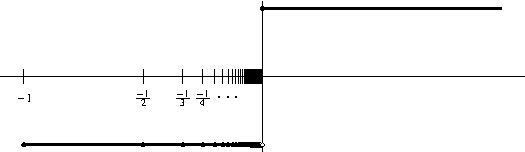
\includegraphics{../figures/jumpdiscont}
\end{center}

\pause
\medskip

Note also:

\medskip

$f(\nicefrac{1}{n}) = 1$ for all $n \in \N$ \wthus $\lim \, f(\nicefrac{1}{n}) = f(0) = 1$.

\pause
\medskip

$f\Bigl(\frac{{(-1)}^n}{n}\Bigr) = {(-1)}^n$.
\end{frame}

\begin{frame}

\textbf{Example:}
Consider the \emph{Dirichlet function}.
\begin{equation*}
f(x) \coloneqq
\begin{cases}
1 & \text{if } x \in \Q , \\
0 & \text{if } x \in \R \setminus \Q .
\end{cases}
\end{equation*}
\pause
$f$ is discontinuous at all $c \in \R$.

\pause
\medskip

Proof:
For $c \in \Q$, take $\{ x_n \}$ in $\R \setminus \Q$ such that $\lim\, x_n = c$.

\pause
$f(x_n) = 0$ ~\thus~ $\lim\, f(x_n) = 0$,
\quad but $f(c) = 1$.

\pause
\medskip

For $c \in \R \setminus \Q$, take $\{ x_n \}$ in $\Q$ such that $\lim\, x_n = c$.

\pause
$f(x_n) = 1$ ~\thus~ $\lim\, f(x_n) = 1$,
\quad but $f(c) = 0$.
\qed

\end{frame}

\begin{frame}

\textbf{Q:}
Does there exist a function continuous at all irrational numbers, but
discontinuous at all rational numbers?

\pause
\medskip

\textbf{A:} Yes.

\pause
\medskip


\textbf{Example:} (\emph{Thomae function} or \emph{popcorn function}).

Define $f \colon (0,1) \to \R$ as
\begin{equation*}
f(x) \coloneqq 
\begin{cases}
\nicefrac{1}{k} & \text{if } x=\nicefrac{m}{k}, \text{ where } m,k \in \N
\text{ and } m \text{ and } k \text{ have no common divisors,} \\
0 & \text{if } x \text{ is irrational.}
\end{cases}
\end{equation*}

\begin{center}
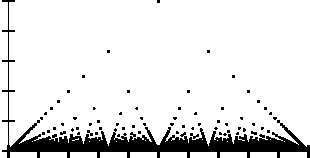
\includegraphics{../figures/popcornfig}
\end{center}

\pause
\medskip

\emph{Claim: $f$ is continuous at every irrational number and discontinuous at every
rational number.}

\end{frame}

\begin{frame}

Proof:
Suppose $c = \nicefrac{m}{k}$.

\pause
Take a sequence $\{ x_n \}$ in $\R \setminus \Q$ such that $\lim\, x_n = c$.

\pause
Then $\lim\, f(x_n) = \lim \, 0 = 0$, but $f(c) = \nicefrac{1}{k} \not= 0$.

\pause
\thus \quad $f$ is discontinuous at $c$.

\pause
\medskip

Now let $c$ be irrational, so $f(c) = 0$.

\pause
Take a sequence $\{ x_n \}$ in $(0,1)$ such that $\lim\, x_n = c$.

\pause
Given $\epsilon > 0$, find $K \in \N$ such that $\nicefrac{1}{K} < \epsilon$.

\pause
If $\nicefrac{m}{k} \in (0,1)$, then $0 < m < k$.

\pause
Only finitely many such numbers where $k < K$.

\pause
As $\lim\, x_n = c$, any $x \not= c$ appears at most
finitely many times in $\{ x_n \}$.

\pause
Hence,
$\exists$ $M$ such that for $n \geq M$, all the numbers $x_n$
that are rational
have a denominator larger than or equal to $K$.
\pause
\begin{equation*}
\text{For } n \geq M, \quad
\abs{f(x_n) - 0} = f(x_n)
\pause
\leq \nicefrac{1}{K}
\pause
< \epsilon .
\end{equation*}
\pause
\thus \quad $f$ is continuous at irrational $c$.
\qed

\end{frame}

\begin{frame}

\textbf{Example:}
Define $g \colon \R \to \R$ by $g(x) \coloneqq 0$ if $x \not= 0$ and
$g(0) \coloneqq 1$.

\pause
\medskip

$g$ is discontinuous at $0$, but continuous on $\R \setminus \{ 0 \}$.

\pause
\medskip

$x=0$ is called a \emph{removable discontinuity}:

We could redefine $g(0)$ and obtain a continuous function.

\pause
\medskip

The jump discontinuty, $f(x) \coloneqq -1$ for $x < 0$ and $f(x) \coloneqq 1$ for $x \geq 0$,

does not have a removable singularity at $x=0$.

\pause
\medskip

$\displaystyle \lim_{x\to 0} g(x)$ exists \quad $\displaystyle \lim_{x\to 0} f(x)$ does not.

\pause
\medskip

Another thing:

Let $A \coloneqq \{ 0\}$ and $B\coloneqq \R \setminus \{0\}$.

\pause
\medskip

$g|_A$ is continuous, but $g$ is not continuous on $A$.

\pause
\medskip

$g|_B$ is continuous, and $g$ is continuous on $B$.

\end{frame}

\end{document}
